\documentclass{mcmthesis}
\mcmsetup{CTeX = false,   % 使用 CTeX 套装时,设置为 true
        tcn = 0028, problem = A,
        sheet = true, titleinsheet = true, keywordsinsheet = true,
        titlepage = false, abstract = true}
\usepackage{palatino}
\usepackage{lipsum}
\usepackage{amsmath}  
\usepackage{amssymb}
\usepackage{indentfirst} 

\setlength{\parindent}{1.5em}

\title{The Modeling of Credit Scoring System }

\begin{document}
\begin{abstract}
  
The risk of Internet finance is increasingly apparent. 
It is urgent to build a credit scoring model based on the data of internet finance to improve the risk control level. Based on personal credit history and credit behavior data, credit behavior model derived from data mining and mathematical statistics method can predict individual's future credit performance more accurately, improve the efficiency of Internet operation and reduce the credit cost of Internet financial transaction .

We try to construct a credit score model for users by lending information to users and use machine learning model to optimize the performance of credit score based on exploring certain feature engineering.

In feature selection, we employ One-Hot, binning, WOE coding and IV values ​​to extract useful training data from user's data as much as possible.

In the model, we use the basic model of machine learning logistic regression and decision tree for binary training. Performance is less than ideal in logistic regression, although commercial credit ratings are mostly logistic regression. However, under given data conditions, the model is weaker than the decision tree.

With the same characteristics, the decision tree model can achieve better credit score performance. Thus, it can be seen that in the case of weak data, the decision tree may have better performance than logistic regression in modeling credit score. Today's mainstream credit scoring model may have many enhancements without losing the benefits of interpretability.
\begin{keywords}
credit scoring; logistic regression; WOE; IV
\end{keywords}
\end{abstract}
\maketitle
\tableofcontents
\newpage
\section{Introduction}
\subsection{Restatement of Problem}

With the continuous improvement of Internet technology and the increasing number of its users, Internet Finance emerges as the times require. At present, it has been springing up, showing a variety of business models and operation mechanisms. It has advantages which have no for other traditional financial , such as the Internet financial institutions can break through the time and geographical constraints,  provide more efficient financial services for the financing needs of customers on the Internet,  use Internet technology, accelerate business processing speed, and give users a better service experience. But at the same time, risks of Internet financial have raised and become more and more, for example, there are problems such as credit risk and user fraud, there is the urgent need to improve the level of risk control by using the Internet financial data,such as to construct a credit scoring model identification and use the model for effective user level for Internet users.

Credit bureaus can collect the abundant information data by making use of  the Internet, use various data processing methods and data modeling skills, and establish a comprehensive credit evaluation model. At the same time the massive and rich data in the personal credit history and credit behavior based on ones , obtain credit behavior model by using data mining and statistical method,  get more accurately the prediction of the future performance of personal credit, improve the efficiency of operation of the Internet,reduce the cost of credit for the Internet financial transactions ,and be able to estimate the risk of Internet consumer credit. The Internet is an important tool which is irreplaceable in financial institutions . Therefore, the establishment of a precise credit scoring system is of great significance for the Internet financial enterprises. For this problem, the historical business data of a loan institution is given as the original data. The following tasks are completed:
\begin{itemize}
\item it is necessary to extract the main factors that affect the user's credit based on the given data.
\item to contact related macroeconomic data to study the impact of user credit in the macro economic environment.
\item using data mining and other methods, construct the model variables ,  formulate credit rules , establish credit evaluation models , and predict default conditions by models which you make.
\item using the established model to analyze the type of default: the objective type (due to the economic environment or the objective conditions) and the subjective type (the conditions are also deliberately not returned).
\end{itemize}
\subsection{Problem Background}

With the continuous development of Internet technology, its influence has permeated every aspect of life. Internet finance has come into being. Compared with traditional finance, Internet finance has the advantages of favoring people. For example, it achieves faster business processing speed, breaks the time and space constraints, provides faster and more convenient financial services and brings better user experience Service experience. However, at the same time, the risks it brings are becoming more and more obvious. For example, credit risk and user fraud, in this context, a set of perfect and effective credit scoring system is particularly important.
\subsection{Our Work}
Credit scoring is based on customer credit history data, using a certain credit score model, get different grades of credit scores. Depending on the customer's credit score, the creditor can analyze the customer's likelihood of repaying on time. Although creditors can also get the result of such analysis by analyzing the customer's credit history, the use of credit scores is faster, more objective, and more consistent.

Given that Logistic regression algorithms are often used in today's commercial credit scoring models, we mainly try this algorithm and decision tree algorithms to train, focusing on data cleaning and variable selection and construction. Some of the choices for variable selection are mainly the screening of credit scores commonly used in the industry. For the given data, we mainly do the following thinking:
\begin{itemize}
\item Which of these customer data sets is unusable.
\item What is the ratio between good and bad customers, how to deal with imbalances.
\item The amount of data itself is not large, how to make the model more fully trained.
\item How to evaluate data to promote model training.
\item Some of the data to do some conversion, making it more suitable for training.
\item Training algorithm itself parameters should be adjusted to the problem.
\end{itemize}

\section{Assumptions}
\begin{itemize}
\item Assume that the historical business data of the lender is stable and trustworthy
\item Assume the default is not affected by emergencies
\item Assume that all borrowers have good credit history before
\end{itemize}

\section{Natations}
\begin{tabular}{cc}
\toprule
Symbol & definition\\
\hline
$TP$ & real case \\
\hline
$FP$ & False Positives\\
\hline
$FN$ & false counsel\\
\hline
$TN$ & True Counter Example\\
\hline
$i$ & Subscripts for various variables \\
\hline
$woe_i$ & a box of evidence weight \\
\hline
$WOE$ & Weight of Evidence \\
\hline
$w$ & weight \\
\hline
$b$ & offset or constant \\
\hline
$\mathbf{w}$ & weight vector \\
\hline
$IV_i$ & Variables The amount of information in a bin \\
\hline
$IV$ & Information value \\
\hline
$B_i$ & the number of bad clients \\
\hline
$B_T$ & Total number of bad clients \\
\hline
$G_i$ & number of good customers \\
\hline
$G_T$ & the total number of good customers \\
\hline
$TPR$ & In all samples that are actually positive, the ratio correctly judged as positive\\
\hline
$FPR$ & In all the negative samples, the ratio of false positives\\
\hline
$p_i$ & The probability of the i-th item\\
\hline
$H$ & measures the uncertainty of random variables\\
\hline
$Gini$ & Gini index (Gini impure)\\
\hline
\end{tabular}

\section{Data Processing}
\subsection{Data Screening}
The amount of data is large, so our priority is to filter the data based on its completeness and validity.\\

First, we screen the data of 30,000 historical business data provided by the lender:\\
\begin{itemize}
\item Since tag attributes are crucial and can not be completed, we delete all business data that did not indicate a default.
\item In the analysis of the attributes, we found that there are a large number of missing attributes of AGENT and salary level in the data, in which the salary level can be complemented because it is a numerical attribute with continuous meaning. For AGENT, because it is text type data and Did not find it related to other attributes, so we choose to delete AGENT this attribute.
\end{itemize}

\subsection{Data Merging}
\begin{itemize}
\item When processing the data we found that the education level variables, there are college and below, junior high school and junior high school, the four classification of repeated phenomena, which are repeated graduate, doctoral and master's degree and more than three kinds of classification, so we will and specialist and below master degree or above and two classification.
\item At the same time, we found that two kinds of definitions of divorce and divorce were duplicated in the marital status. We merged them into divorce. At the same time, we considered the semantic description of marital status. We merged the widowhood into divorce and merged the other into the unmarried.
\item For borrowing time, we provide data from January to June 2017, so we combine it into 6 categories representing 6 months to facilitate later use. .
\item For the working provinces, we divide the provinces into four large areas, the eastern, the northeast, the central and the western regions, according to the division of the sixteen regions of the Communist Party of China and the development of the provinces in the past year (Figure).
\end{itemize}

\begin{figure}[h]
\large
\centering
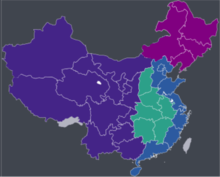
\includegraphics{map.png}
\caption{National Economic Zone} \label{fig:National Economic Zone}
\end{figure}

\subsection{Missing Value Processing}

In statistics, missing data occur when no data value is stored for the variable in an observation.Missing data are a common occurrence and can have a significant effect on the conclusions that can be drawn from the data.

In the data we use, there is a large amount of data that is missing a salary grade variable, and we consider doing so due to the lack of a large amount of data and the variable is a numeric data with a continuous relationship. We have statistics on the available data and found that the overall data is normally distributed.
\newpage
\begin{figure}[h]
\small
\centering
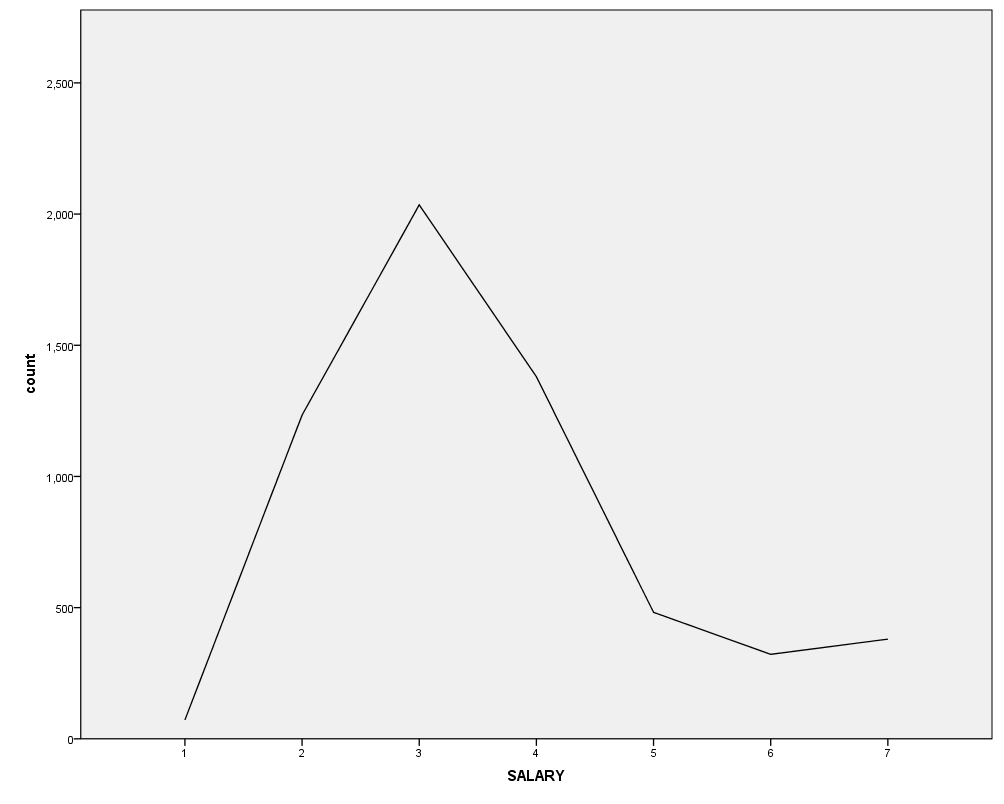
\includegraphics[width=10cm]{sosl.png}
\caption{The level of salary statistics} \label{fig:The level of salary statistics}
\end{figure}

Then we consider that the pay scale may be influenced by the level of education and the work area, so we will analyze it on the assumption that different education levels and pay scales are different from those in the work area.

\begin{figure}[h]
\small
\centering
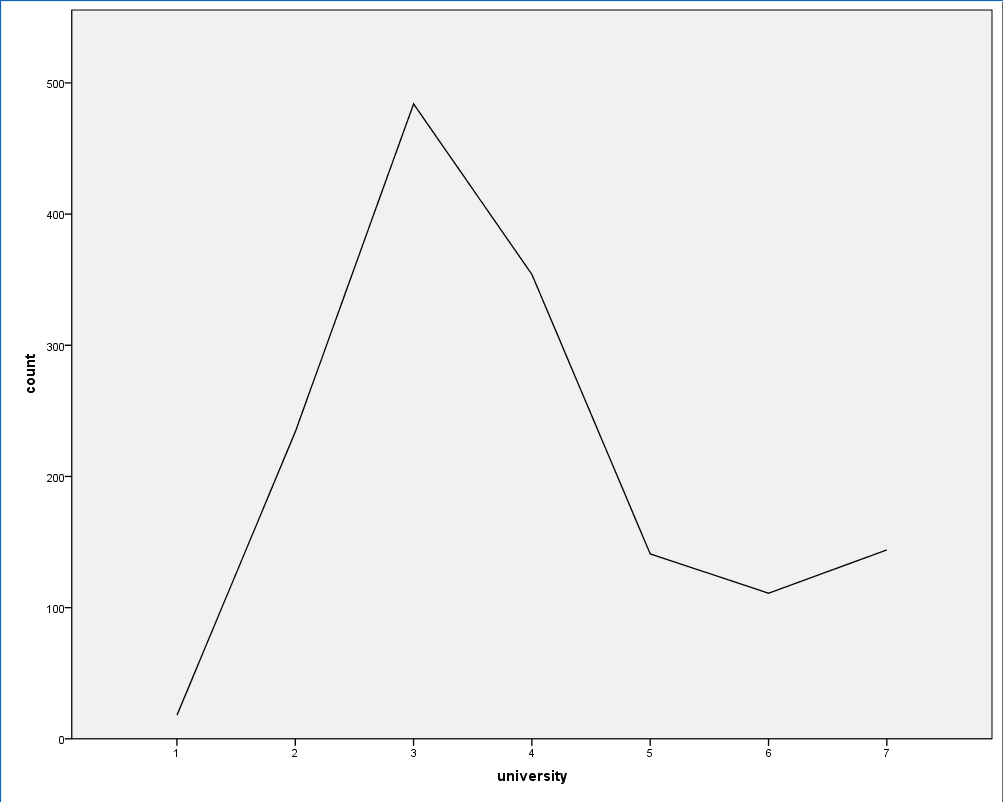
\includegraphics[width=10cm]{un.png}
\caption{Undergraduate education level of the amount of salary level statistics} \label{fig:Undergraduate education level of the amount of salary level statistics}
\end{figure}

We found that at different levels of education, salary levels are basically normal distribution, so taking the level of compensation at different levels of education found. The proportion of high salaries at the educational level of masters and above is higher than that of other education levels. However, taking into consideration the low level of data in this level of education, The horizontal approximation is seen as a normal distribution.
\newpage

\begin{figure}[h]
\small
\centering
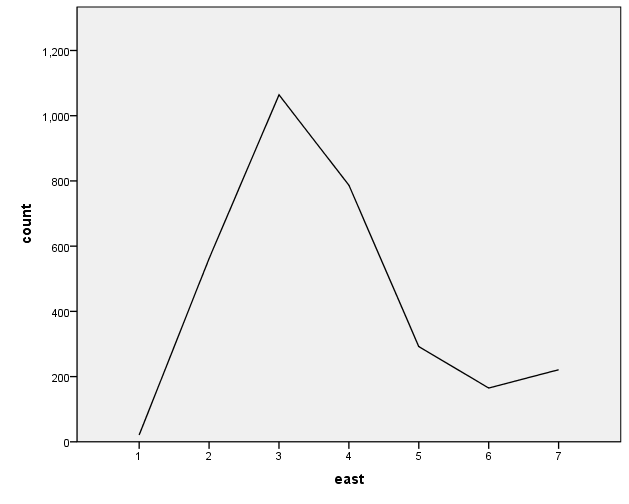
\includegraphics[width=10cm]{east.png}
\caption{The eastern region of the amount of salary level statistics} \label{fig:The eastern region of the amount of salary level statistics}
\end{figure}

For different workplaces, we also analyze their salary levels.

We also found that in all workplaces, all salary levels are normally distributed, so we conclude that the salary level in this data is normally distributed, with no educational level or work area impact.

In this regard, we take the average and mode and draw the relevant charts for a preliminary analysis.

\begin{figure}[h]
\small
\centering
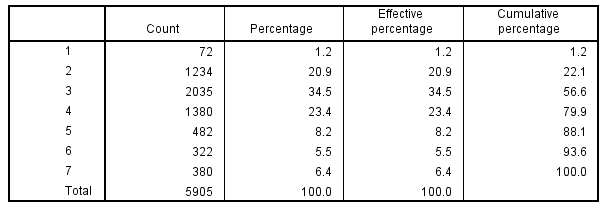
\includegraphics[width=12cm]{sp.png}
\caption{The amount of salary level statistics} \label{fig:The amount of salary level statistics}
\end{figure}

We can see that the average is 3.58 and the mode is 3. Taking into consideration and facilitating our later use, we decided to set the missing value of all pay levels to 3.

\subsection{Unbalanced Data Processing}
Statistical statistics on the number of data labels found that the number of non-defaults is much larger than the number of defaults (as shown in the figure), which easily leads our model to predict all the results as non-defaulting during training, and the final correctness rate is as high as 0.9 on the surface The actual prediction accuracy of the default is 0, in order to avoid this phenomenon, we under-sampled and oversampled the data processing, making the difference between the two types of data should not be too large
\newline
\begin{figure}[h]
\small
\centering
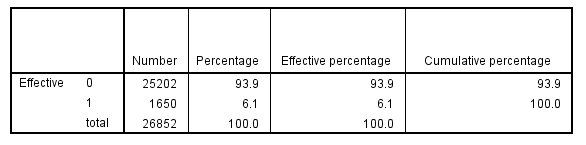
\includegraphics{ttns.png}
\caption{Tag type number statistics} \label{fig:Tag type number statistics}
\end{figure}

\section{Our Model}
Based on available information, consider the current credit scoring model and the industry's interpretative requirements for credit scoring models. Our initial consideration of the model is logistic regression.

The data, the marital status can not simply use the serial number to represent, this will result in some similar marital status but the actual situation is not. The marriage attribute itself is not sequential, so we carried out One-Hot encoding. By the same token, taking into account the rough change of the academic data itself, the order of academic qualifications becomes vague, and we also carry the One-Hot code for academic qualifications. Finally, consider the province data, the province of our data is a 6-digit zip code. It is observed that the left-most 2-digit postcode represents its province, so we converted that data to obtain the customer's province code. Taking into account the large number of provinces in China, we have reviewed the relevant information and found that China is divided into four major economic regions: the eastern region, the northeast region, the central region and the western region. The main contents of economic and social development in various regions are: development in the west, rejuvenation in the northeast, rise in the middle and development in the east. Taking into account the loan, credit score and economy, we divided the provinces data:

Northeast China (Heilongjiang, Jilin, Liaoning, Hulunbeier, Xing'an League, Tongliao, Chifeng, Xilin Gol League in eastern Inner Mongolia Autonomous Region)

Middle region (Shanxi, Henan, Hubei, Hunan, Jiangxi, Anhui)

Eastern China (Beijing, Tianjin, Hebei, Shandong, Jiangsu, Shanghai, Zhejiang, Fujian, Guangdong, Hainan)

Western Region (Sichuan Province, Guangxi Zhuang Autonomous Region, Guizhou Province, Yunnan Province, Chongqing Municipality, Shaanxi Province, Gansu Province, West Inner Mongolia Autonomous Region, Ningxia Hui Autonomous Region, Xinjiang Uygur Autonomous Region, Qinghai Province and Tibet Autonomous Region)

The following is based on the first two digits of the ID card coding:
\begin{itemize}
  \item Northeast: 21,22,23
  \item Middle: 14,41,42,43,36,34
  \item East: 11,12,13,37,32,31,33,35,44,46  
  \item Western Region: 51,45,52,53,50,61,62,15,64,65,63,54
\end{itemize}

In fact, there is no order between provinces, so we once again conducted One-Hot encoding on the data.

After the above steps, the current data should be able to train. However, before training, we still need to do some characteristic engineering.

We use a method commonly used in the industry for screening based on IV values.

First introduce concepts and formulas.

The full name of IV is Information Value, find the value of wo first wo value, here also introduced the concept of woe.

WOE (weight of Evidence) is actually an influence on the proportion of default when a certain value is taken from an independent variable. After WOE encoding, the independent variable actually has some standardized nature, that is, each value of the independent variable Can be directly compared (between WOE), and various values ​​between different independent variables can also be directly compared by WOE. Furthermore, we can study the variation (fluctuation) of the WOE value in the independent variable and construct the contribution rate and relative importance of each independent variable in combination with the coefficients fitted by the model. In general, the larger the coefficient, the greater the variance of woe, the greater the contribution of the independent variable (similar to some variance contribution), which can also be intuitively understood.

To conclude, the process of independent variables (including coding and filtering) is largely based on the evaluation of the effects of univariate models when doing credit scoring models. In this evaluation process, ROC and IV examine the impact of independent variables on the target variables from different perspectives. Based on this investigation, we used the WOE value to encode the categorical independent variables so that the independent variables can be more intuitively understood The role of variables and direction, while enhancing the prediction effect.

The advantages of WOE transformation: Improve the predictive effect of the model and improve the comprehensibility of the model.

First group variables (how to say later), then for each group i, for the i group:
\[woe_i = \ln(\frac{B_i / B_T}{G_i / G_T})\eqno (1)\]

For example, if only the absolute value of woe is summed up, if some groups have a small number of A groups and a large number of B groups (obviously such a group is unreasonable), this is a small woe value of B and a large group A , Sum woe will not be small, apparently so unreasonable.
\[IV_i = (\frac{B_i}{B_T} - \frac{G_i}{G_T}) * woe_i\eqno (2)\]
\[IV = \sum_{k=0}^n IV_i\eqno (3)\]

Finally, we can sort the variables according to the size of each variable IV value. The greater the IV to retain.

\begin{table}[h]
\centering
\caption{Predicted based on IV value}
\begin{tabular}{c|c}
\hline
IV & Predictive Ability\\
\hline
<0.03 & NAUGHT\\
\hline
0.03 - 0.09 & LOW\\
\hline
0.1 - 0.29 & MIDDLE\\
\hline
0.3 - 0.49 & HIGH\\
\hline
>= 0.5 & VERY HIGH\\
\hline
\end{tabular}
\label{tab1}
\end{table}

Take the credit scorecard modeling scenario as an example: X is the customer sample field, Y indicates whether the customer is overdue, where Y = 1 means overdue, Y = 0 means not overdue. We want to be able to use the information known to our clients to predict the probability of overdue after the customer borrows, in order to decide whether to lend.

\begin{table}[h]
\centering
\caption{IV of the Attribute}
\begin{tabular}{c|c}
\hline
Attribute & IV\\
\hline
LOAN\_DATE & 0.112\\
\hline
IS\_LOCAL & 0.032\\
\hline
WORK\_PROVINCE' & 0.233\\
\hline
EDU\_LEVEL & 0.025\\
\hline
MARRY\_STATUS & 0.012\\
\hline
SALARY\_LEVEL & 0.173\\
\hline
HAS\_FUND & 0.000\\
\hline
\end{tabular}
\label{tab2}
\end{table}

We calculate the WOE value of each attribute field for the previous data, and then calculate the corresponding IV value based on the WOE value. IV measures the amount of information on a variable. IV can be used to represent the predictive power of a variable.

\section{Analysis of the Result}
Through the prediction of the test data, the accuracy rate is 0.74, the recall rate is 0.51, and the overall prediction accuracy rate is 0.62 (see picture). Overall, the effect is not good. However, the issue of default assessment with credit rating, the more emphasis on recall rate, so the recall rate of 0.51 basically meet the demand.
\newpage
\begin{figure}[h]
\small
\centering
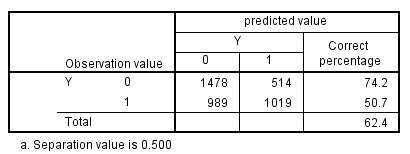
\includegraphics[width=12cm]{result.png}
\caption{result analysis} \label{fig:result analysis}
\end{figure}

Draw its ROC curve can be seen that the model can easily predict whether the default. However, in the process of model establishment, the model can only detect the correctness of the model to a certain extent because the quantity is less than the real one.
\begin{figure}[h]
\small
\centering
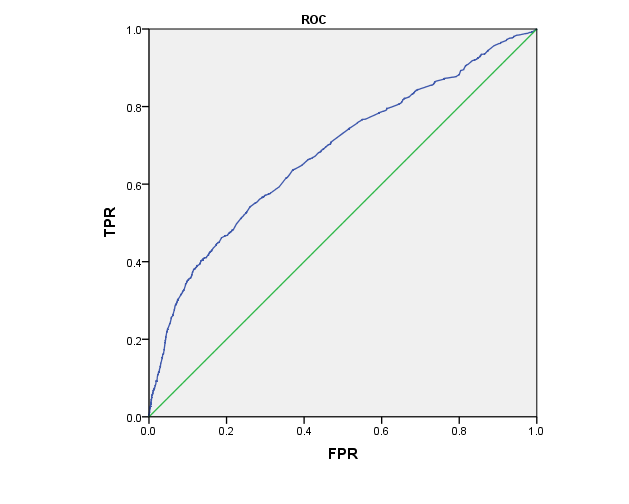
\includegraphics[width=12cm]{ROC.png}
\caption{ROC} \label{fig:ROC}
\end{figure}

\section{Model Evaluation}
\subsection{Advantage}
\begin{itemize}
\item The established prediction model can be closely connected with the actual situation, and solve the problem with the actual situation, making the model has good versatility and promotion
\item The model is calculated using a professional mathematical analysis software, a high degree of feasibility
\item The data was carefully handled, re-encoding variables, they use the latter model
\item Quantitative analysis of many influencing factors involved in the model, which makes the thesis persuasive
\end{itemize}
\subsection{Disadvantage}
\begin{itemize}
\item No detailed correlation test for variables in the data, leading to a higher significance for some of the variables
\item For this problem, we introduce more external materials and create less ourselves
\item due to the time, not a good grasp of the thesis center, people feel a bit scattered papers, failed to make a comprehensive revision
\end{itemize}
\subsection{Improvement}
\begin{itemize}
\item due to the time, the reference is not perfect, the follow-up can be slowly adjusted, and simplify the model
\item using a single logistic regression model is not effective, follow-up can use adaboost and other integrated learning will be a number of simple model collection
\end{itemize}

Logistic regression is strongly data dependent on this problem, given the poor performance of logistic regression, we then use the decision tree algorithm to train and do some fine tuning.

Common advantages of decision tree algorithms are as follows:
\begin{itemize}
\item high classification accuracy
\item The generated model is simple
\item Good robustness to noise data
\end{itemize}

We choose the gini coefficient as the basis for the division, the Gini index (Gini Impurity): the probability of a randomly selected sample being mispicked in the sample set.

The overall data as before, adjusted the following test:\\
Information entropy:\\
\[H (X) = - \ sum_ {i = 1} ^ n p_i \ log (p_i)\eqno (4)\]
Gini Coefficient:\\
\[Gini (p) = \ sum_ {k = 1} ^ K p_k (1 - p_k)\eqno (5)\]
\newpage
\begin{figure}[h]
\small
\centering
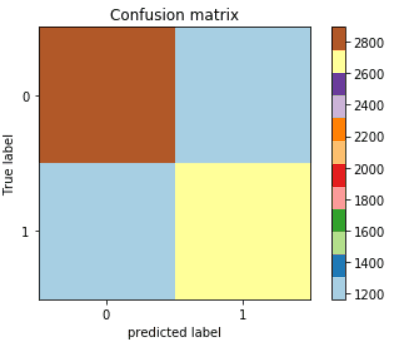
\includegraphics[width=12cm]{matrix.png}
\caption{Confusion Matrix} \label{fig:Confusion Matrix}
\end{figure}

Calculation can be a variety of evaluation indicators are as follows:
\begin{table}[h]
\centering
\caption{Evaluation Index}
\begin{tabular}{c|c}
\hline
acc & 0.691375\\
\hline
recall & 0.669119512814\\
\hline
precision & 0.693582325092\\
\hline
\end{tabular}
\label{tab2}
\end{table}]

As can be seen, relative to the previous logistic regression, the overall increase is larger. at this time,
The impact of a relatively small sample of bad clients has been greatly reduced. Will not appear always tend to
Evaluate as a good customer. It appears that over-sampling and under-sampling play a more significant role in the decision tree.
The common credit rating indicators available on the web show that 60\% is acceptable and 70\% is good.
\begin{figure}[h]
\small
\centering
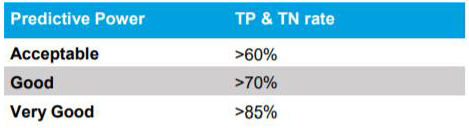
\includegraphics[width=12cm]{ei.png}
\caption{Matrix evaluation index} \label{fig:Matrix evaluation index}
\end{figure}

% \begin{Theorem} \label{thm:latex}
% \LaTeX
% \end{Theorem}
% \begin{Lemma} \label{thm:tex}
% \TeX .
% \end{Lemma}
% \begin{proof}
% The proof of theorem.
% \end{proof}

\begin{thebibliography}{99}
% \bibitem{1} D.~E. KNUTH   The \TeX{}book  the American
% Mathematical Society and Addison-Wesley
% Publishing Company , 1984-1986.
% \bibitem{2}Lamport, Leslie,  \LaTeX{}: `` A Document Preparation System '',
% Addison-Wesley Publishing Company, 1986.
\bibitem{1}\url{https://zhuanlan.zhihu.com/p/27770760}
\bibitem{2}\url{http://news.cnfol.com/guoneicaijing/20180124/25946369.shtml}
\bibitem{3}\url{https://en.wikipedia.org/wiki/Credit_scoret}
\bibitem{4}\url{https://zhuanlan.zhihu.com/p/30026040}
\bibitem{5}\url{https://help.aliyun.com/document_detail/55269.html?spm=5176.10695662.1996646101.searchclickresult.2b4af88cKoTF8e
}
\end{thebibliography}

\end{document}

%% 
%% This work consists of these files mcmthesis.dtx,
%%                                   figures/ and
%%                                   code/,
%% and the derived files             mcmthesis.cls,
%%                                   mcmthesis-demo.tex,
%%                                   README,
%%                                   LICENSE,
%%                                   mcmthesis.pdf and
%%                                   mcmthesis-demo.pdf.
%%
%% End of file `mcmthesis-demo.tex'.
